\documentclass[11pt]{memoir}

\usepackage{import}
\import{../}{gov-style}
\addbibresource{../thesis.bib}

\begin{document}
\section{The value of espionage}
\subsection{Connecting theory to empirics}
I draw two major conclusions from the evidence presented in this thesis, one regarding espionage norms generally and the other about establishing norms through cyber policy. This section will connect the theoretical basis for espionage norms from Chapter 2 with the empirics from Chapters 3 and 4. Not only does the process tracing employed in the empirical chapters support the defensive realist hypothesis, it suggests that the nuclear age further induced states to solve the security dilemma by setting the stakes for failure at apocalyptic levels. The final section will use the lessons from space policy to make a case for why the United States should push for an international accord that explicitly protects the peaceful uses of cyberspace. For cyber espionage to remain mutually valuable, it cannot be used as a justification for cyber weapons. The United States has the most to gain from eliminating cyberspace as a domain for conflict and the most to lose if it fails to do so.

The first chapter presented the puzzling state of cyber policy today, where policymakers often categorize damaging cyber attacks as traditional espionage and decline to impose diplomatic consequences as a result. I theorized that the United States limited its diplomatic response to cyber espionage because espionage has traditionally served a purpose that it was interested in preserving. Then I developed a intellectual framework to explain that purpose using Glaser's defensive realism: security-seeking states have a rational incentive to solve the security dilemma and espionage norms provide a means with which to do. Even if espionage norms put one state at a relative disadvantage, maintaining them leaves the state more secure than it would be otherwise; in this formulation, the alternative is an arms race that leaves all states worse off.

President Eisenhower did not use the term defensive realism when he approved Project Aquatone in 1954---the same year that Charles Glaser was born---but its premise perfectly describes his approach to intelligence. Under his leadership, the United States used technological intelligence to great de-escalatory effect; he resisted alarmist demands from the military-industrial complex and encouraged an international norm protecting the peaceful uses of space. Despite causing an uproar at the Paris Summit, Khrushchev acquiesced to these developments; the Soviet Union built its own spy satellites and the two states settled into a cooperative equilibrium. The tacit accord on mutual reconnaissance---which became a legal accord in 1972---led to relative gains in American security, but absolute gains for both the the US and the USSR.

Both Eisenhower and Khrushchev cooperated to minimize the punishment for espionage, but because Khrushchev's decision is more counterintuitive, the argument that both states employed defensive realism would be even stronger if he had articulated his approach to intelligence in analogous terms, the way Eisenhower did. Unfortunately, his memoirs often obfuscate on issues of intelligence, leaving his son Sergei to fill in the gaps and correct the misrepresentations. That reluctance is nonetheless informative, because it correlates with how political figures interested in preserving espionage norms often discuss intelligence---reassuring the public that they did everything possible to counteract ``outrageous'' intrusions while quietly preserving the incentives to commit them. Sergei's annotations provide important factual context even if they cannot conclusively establish his father's motivations. Given the secrecy of Soviet society, that is about as good as can be expected. Nikita Khrushchev secretly dictated his memoirs into a tape recorder, hid the tapes from the KGB, and had them smuggled to the West, all while living in housing provided by the people who had deposed him---he had few opportunities for candor.

\subsection{Miscalculation the nuclear age}
Solving the security dilemma is a valuable goal for any security-seeking state, but it takes on increased importance as the potential war becomes more dangerous, and absolutely nothing was more threatening to either the US or the USSR than the possibility of general nuclear conflict. The evidence suggests that the United States would not have been as successful at translating espionage norms to technology had it attempted to do so before the development of the atomic bomb. Artificial satellites were developed concurrently with ballistic missiles but planes are obviously much older---so why did no state attempt to build a plane for peacetime reconnaissance before the Second World War? Such a plane would not have flown as high as the U-2, but it could have replicated the photography-only design. The answer is intuitive: a spy flight directly over Germany in 1936 would almost certainly have been interpreted as an act of war.

A hypothetical overflight in Germany sounds faintly absurd---even though the US did exactly that to Russia in 1956---because the application of espionage norms to technical intelligence is inextricably linked with the fear of nuclear war. The United States was driven to technical intelligence because its leaders were terrified of a ``nuclear Pearl Harbor.'' U-2 photography was needed to disprove the (nuclear) bomber gap and satellite photography did the same for missile gap. Technical intelligence directly solved one of the key barriers to bilateral nuclear arms control. Policymakers were looking for reasons not to have to launch a nuclear weapon and espionage was uniquely suited to provide those reasons---but it only worked because they could count on their opponents being equally averse to nuclear war.

Espionage norms are sustained by the same logical structure that has prevented nuclear war for the last 75 years. The decision matrix for espionage from Chapter 2 is functionally equivalent to a situation of mutually assured destruction. Were either state to punish espionage with unprecedented harshness, then they are assured that the other state would do the same, limiting the flow of information. The same logic applies to nuclear war: no matter which state attacks first, the other state is guaranteed to respond. In both cases, the two opponents are playing tit-for-tat; the only long-term outcomes are mutual cooperation (open flow of intelligence, relative peace) or mutual defection (closed intelligence, nuclear war).

\begin{table}[ht]
\centering
\setlength{\extrarowheight}{2pt}
\begin{tabular}{cc|c|c|}
  & \multicolumn{1}{c}{} & \multicolumn{2}{c}{USSR}\\
  & \multicolumn{1}{c}{} & \multicolumn{1}{c}{Hold Fire}  & \multicolumn{1}{c}{Nuclear Strike} \\\cline{3-4}
  \multirow{3}*{USA}  & Hold Fire & \makecell{~\\No nuclear war \\~} & \makecell{\\~~~Soviet first-strike~~~~\\ $\downarrow$ \\ Total nuclear war\\~} \\\cline{3-4}
  & Nuclear Strike & \makecell{\\American first-strike \\ $\downarrow$\\Total nuclear war\\~} & \makecell{~\\ Total nuclear war \\~} \\\cline{3-4}
\end{tabular}
\caption{Nuclear strike decision matrix}
\label{nuclear-war-matrix}
\end{table}

Ending the traditional tolerance of espionage would not immediately lead to nuclear war, but the threat of nuclear war is always present in the decision to preserve it. The historical connection between espionage and arms control suggests that states realize that restricting the former makes trust more difficult and miscalculation more likely. The scenarios in this thesis demonstrate a consistent bias towards a world in which every actor is making the most informed decisions possible, precisely because it reduces the risk of miscalculation. In the nuclear age, miscalculation could be fatal, and states recognize that it is always in their best interest not to annihilate life on Earth.

% My conclusion that espionage norms help de-escalate nuclear conflict has a caveat: intelligence is not always used to reduce security tensions---it can just as easily have a neutral, or even negative effect. The most transformative intelligence failure of my lifetime was the 2003 invasion of Iraq, now considered, by virtually all ends of the political spectrum, to have been a colossal mistake. Much of the blame for that mistake rests at the feet of the American intelligence community, which the bipartisan Robb-Silberman Commission determined ``was dead wrong in almost all of its pre-war judgments about Iraq's weapons of mass destruction.''\footcite{commission_on_the_intelligence_capabilities_of_the_united_states_regarding_wmds_final_2005} There is no way to say whether the Second Gulf War would have been more or less likely without that faulty intelligence, but I mention it as a reminder that more intelligence does not always lead to more secure outcomes, and my conclusion should not be interpreted as such.

\subsection{Spying in cyberspace}
This thesis provides a framework to evaluate whether it is wise to maintain a distinction between cyber espionage and other forms of illegal cyber activity---and I conclude the answer is a cautious yes. Even without knowing what the United States is learning from its cyber espionage program, we know what effect espionage has on the international system. The US is likely making more well-informed decisions as a result of cyber espionage and it benefits from a legal regime where all states are doing the same. Espionage between states broadly serves to make miscalculation less likely and cyber espionage is its most modern application.

Based on the evidence available today, it is probably impossible to directly connect American cyber espionage to any form of arms control or nuclear de-esclation. That should not be seen as discouraging---we are only able to make such definitive claims about the photo-reconnaissance techniques discussed in this thesis because they are mostly obsolete. Much of the information about the U-2 plane and early spy satellites is now declassified; the relevant information about American cyber espionage and modern spy satellites is not. Official memoirs and intelligence histories recount exactly how the Corona intelligence prevented nuclear miscalculation. It will be a long time before we see similarly detailed information about analogous cyber programs.

As long as the intelligence gained from cyber espionage is used in ways that are typical of espionage, then the manner by which it was obtained is mostly irrelevant. Military analysts are bound to argue that the US is losing competitiveness from theft of military technology. Such losses, however, fit easily within the bounds of traditional espionage. The quality of the military technology that has been stolen is not unique to this era; imagine a world without Soviet penetration of the Manhattan project, causing the Soviet Union to develop atomic weapons even just a few years later. While Chinese theft of military technology is no doubt significant, when it is used exclusively for military purposes, its impact is limited to an arena where the benefits of defensive realism still apply. Were the US military presented with the option to end espionage on both sides, the evidence presented here makes it seem highly unlikely that they would choose to do so.

The intelligence profession is changing rapidly and its norms will no doubt have to adapt as well. Worries the about scale of cyber espionage are understandable---22 million documents!---but they are also reciprocal and, in the internet age, unavoidable. What would have been a bulletproof cover story 20 years ago can be disproved withing a few minutes of searching the internet.\footcite{lucas_spycraft_2019} Society is only just beginning the grapple with how to handle the massive amount of data that is collected on every individual who maintains an presence online. The implications of this evolution extend far beyond espionage.

\section{Peaceful uses of cyberspace}
\subsection{The importance of norm entrepreneurship}
If American cyber policy already creates a diplomatic exception for traditional espionage, and that exception is worth maintaining, then why does the United States seem to struggle much with discouraging various types of cyberattack? I can only address a small part of that problem, but from the perspective of intelligence, it appears that the United States has been reluctant to act as a norm entrepreneur. Even though its methods of responding to cyberattacks are relatively consistent---attacks that go beyond traditional espionage receive harsher punishments---the stated framework by which it makes those decisions is vague. That makes it difficult for the US to export its cyber policy and encourage international norms to develop in accordance with it.

The opposite was true during the space race---the Eisenhower administration set a clear strategic goal and a developed a long-term plan to attain it. The US built reconnaissance craft and modeled their appropriate use. It worked to develop an international norm that would tacitly accept reconnaissance alongside an international legal framework that would properly legitimize it. In public forums, administration officials made forceful arguments that observation ought to be permitted and westernization shunned. The American success is stunning---Cold War space policy not only secured the use of outer space for peaceful reconnaissance, it kept outer space free of weapons entirely.

The peaceful uses of space provide a blueprint for how the US could promote an analogous norm in cyberspace. Were American policymakers so inclined, they could define a peaceful uses of cyberspace norm that, like in outer space, permits militarization but not weaponization. Compliant states could not use unauthorized access to digital systems for anything more than surveillance---kinetic damage, like overheating hard drives and corrupting data, would be strictly off-limits. The US could essentially take its existing schema for responding to cyberattacks, define its bounds more rigorously, and promote its adoption as a universal standard---either thorough an international legal regime, or a more informal series of agreements between great powers.

The US does know how to use its enforcement mechanisms to establish norms in cyberspace. Even though that accord has not been completely successful, it established that economic espionage in cyberspace is US policy goal. That clarity matters; the Chinese government does not entirely abide by the 2015 agreement, but because the agreement exists, the US has a powerful justification for its retaliatory measures.\footcite{bartz_u.s._2018} Naval Academy professor Martin Libiki describes it as ``the first norm that the United States (successfully) fought for: cyber espionage is acceptable unless the results are used to help a country’s firms compete.''\footcite{libicki_coming_2017} The norm against economic espionage is contested, but it undoubtedly exists.

\subsection{It's never too late for now}
It is time for the United States to take an active role in developing the norms of cyberspace.

Right now the United States has no such vision, and, more troublingly, it seems to be agnostic about advocating for a norm that prohibits using the internet as a weapon.

% The US had. The US \emph{does} make a distinction between attacks that cause physical damage


% Economic espionage ``Economic espionage is 10x worse than whether or Russian can steal information about our F-35 fighter. The ability to counter our economic wealth is significant. ''

% This is does not ensure that the norm will ultimately be adopted---but sets the US up to
having some permissible espionage makes the limits seem more reasonable



% kinetic cyberattacks have happened, iran vs saudi, nk vs us, stuxnet

Were it so inclined, the US could encourage a norm that  As with reconnaissance satellites, the demand for intelligence is too great to expect that state-sponsored hacking can be eliminated entirely; some malicious cyber activity will inevitably take place. If it maintains a clear vision, however, the success of American space policy might be replicable in cyberspace.

Allowing the cyberspace to become a normalized area for combat would be a massive mistake. Offensive cyber operations are


% For the United States to maintain the cooperative equilibrium of espionage it must state what kind of cyber activity it will not tolerate with much greater granularity than it currently does---then forcefully respond to cyber activity that does not play by the rules of the game.

% The one area in which the US has been relatively


% \subsection{Don't shoot me I'm only the spy pilot}

% The evidence of the empirical chapters makes a strong case that framing the U-2 and Corona projects as intelligence efforts---in everything from their design to the bureaucracy that administered them---effectively reduced the diplomatic consequences when that technology was discovered, but it should be noted that the evidence is circumstantial. We know that Eisenhower thought it important that the CIA run the U-2 program instead of the Air Force, and we know that the USSR did not bomb the base from which the U-2 was launched, in retaliation for the deeply illegal overflight. It is tough to say that one caused the other. We know that the USSR traded Gary Powers for a spy, and the Khrushchev deceitfully downplayed the frequency of reconnaissance overflights in his memoirs. Khrushchev's attitude towards the incident is very similar to how states routinely minimize the frequency and effect of espionage against them, but without a quote saying as much, it would impossible to assign him that exact motive.

% Whatever other circumstances might have influenced the Soviet response to American technical reconnaissance, we know for certain that Eisenhower sought to make build a clear association between between technological reconnaissance instruments and human spies, and that he was successful. The U-2 essentially invented the term ``spy plane,'' and appeared as such in \emph{The New York Times}. In the early days of the Corona project, the Soviets press decried the American attempt at ``espionage from space.'' Even if a norm against ASATs had not followed, the United States had already succeeded in associating their new technology with a set of norms that limited how much it could be punished. This association is not an exact science; The rules of the game are entirely comprised of tradition and familiarity, and when you replace a human with a manned aircraft, or a manned aircraft with a beeping ball of metal, it looks less like something that intelligence professionals are used to responding to.

% Eisenhower maximized the odds that the Soviet Union would see spy planes and spy satellites as espionage equipment, but the margin of his success was slim. One does not know what would have happened diplomatically had it turned out that the U-2 was also capable of dropping a bomb, but we do know that American and Soviet restraint on weaponized satellites was decisive in preserving the freedom of space. Deploying an orbital bomb or an ASAT would have completely changed the space race. Both sides were able to agree with spy satellites did not constitute a provocation, but had either side deployed a space weapon that clearly did, then there is no guarantee that spy satellites would have been immune from the backlash. Preserving the norms of espionage in space required that space not be used for weapons.

Establishing limitations on how they can be used!

\subsection{American reliance on technology}
Today, space has been thoroughly militarized, but not weaponized. The difference between the two is significant; weaponization requires the placement of space-based devices that have destructive capacity, such as an orbital satellite loaded with nuclear bombs, while militarization is simply the use of space-based devices to facilitate military operations.\footcite[p.~3]{mowthorpe_militarization_2004} Currently no one faces the threat of an attack originating from space, but an incredible number of more traditional American military capabilities rely on the network of satellites. According to the official government website, The Global Positioning System (GPS) alone is used by the DoD for precision guided munition strikes, force tracking, search and rescue, and remote piloting of unmanned aerial vehicles.\footcite{national_coordination_office_for_space-based_positioning_navigation_and_timing_federal_2018} A fleet of spy satellites, built and maintained by the National Reconnaissance Office since 1961, take high-resolution photos of places Gary Powers could never have reached.\footcite{national_reconnaissance_office_about_2019} The many commercial and civil satellites operated by American entities have military applications as well.


There are a lot of possible targets.\footcite[A few satellites are listed as dual-purpose (i.e. Government/Military), and those are counted twice, once for each purpose. For instance, the data shows that the US is currently operating 830 satellites, while adding up the bars in this chart would give you 966. I made this choice to emphasize the dependency of various social systems on the existing satellite infrastructure.]{union_of_concerned_scientists_ucs_2018}


\begin{figure}[ht]
  \centering
  % Created by tikzDevice version 0.12 on 2019-05-03 23:25:55
% !TEX encoding = UTF-8 Unicode
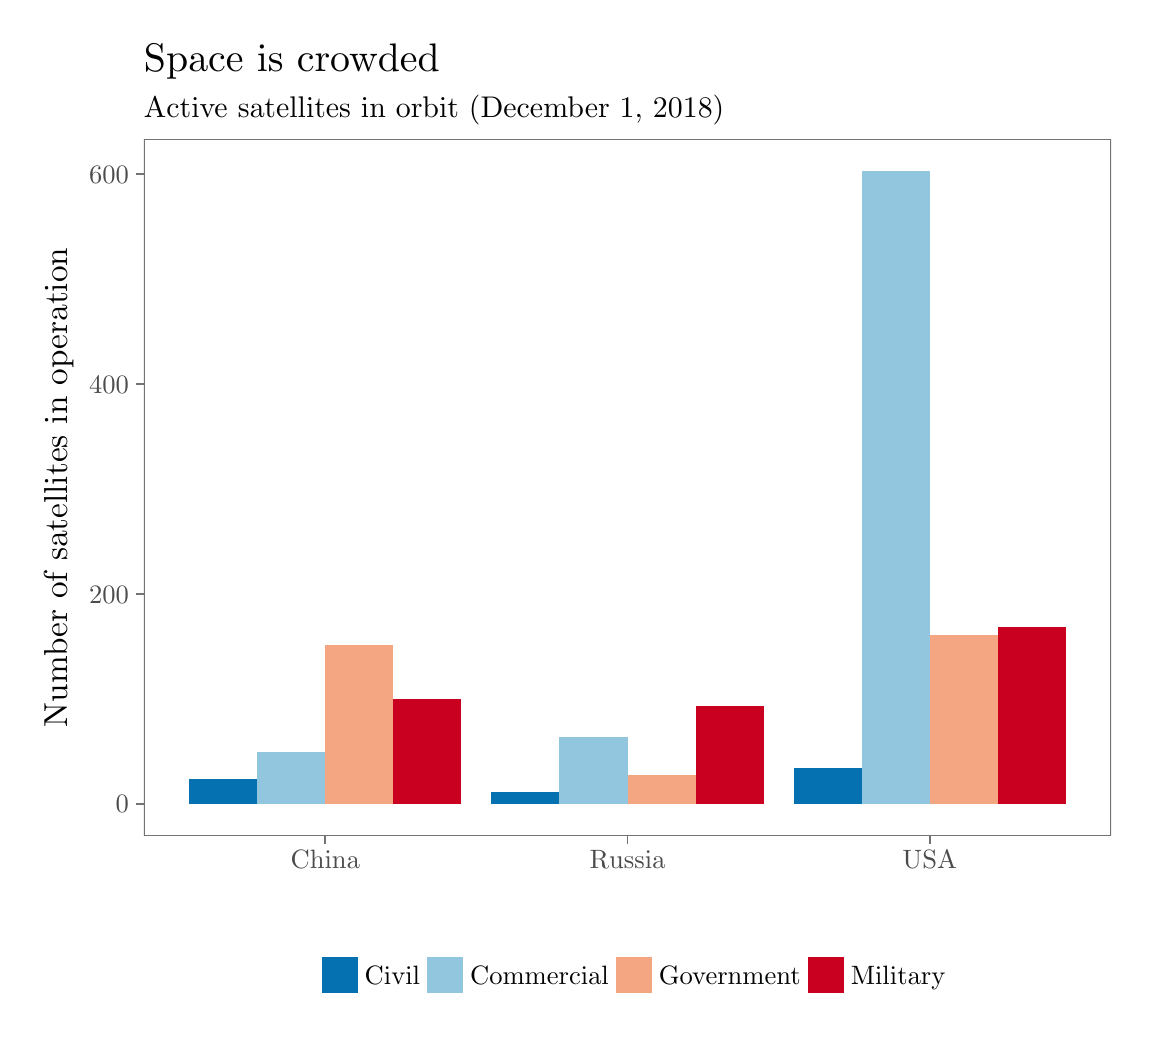
\begin{tikzpicture}[x=1pt,y=1pt]
\definecolor{fillColor}{RGB}{255,255,255}
\path[use as bounding box,fill=fillColor,fill opacity=0.00] (0,0) rectangle (397.48,361.35);
\begin{scope}
\path[clip] (  0.00,  0.00) rectangle (397.48,361.35);
\definecolor{drawColor}{RGB}{255,255,255}
\definecolor{fillColor}{RGB}{255,255,255}

\path[draw=drawColor,line width= 0.6pt,line join=round,line cap=round,fill=fillColor] (  0.00,  0.00) rectangle (397.48,361.35);
\end{scope}
\begin{scope}
\path[clip] ( 42.01, 69.49) rectangle (391.48,320.95);
\definecolor{fillColor}{RGB}{255,255,255}

\path[fill=fillColor] ( 42.01, 69.49) rectangle (391.48,320.95);
\definecolor{fillColor}{RGB}{202,0,32}

\path[fill=fillColor] (132.11, 80.92) rectangle (156.68,118.83);
\definecolor{fillColor}{RGB}{244,165,130}

\path[fill=fillColor] (107.53, 80.92) rectangle (132.11,138.17);
\definecolor{fillColor}{RGB}{146,197,222}

\path[fill=fillColor] ( 82.96, 80.92) rectangle (107.53, 99.50);
\definecolor{fillColor}{RGB}{5,113,176}

\path[fill=fillColor] ( 58.39, 80.92) rectangle ( 82.96, 90.02);
\definecolor{fillColor}{RGB}{202,0,32}

\path[fill=fillColor] (241.32, 80.92) rectangle (265.89,116.18);
\definecolor{fillColor}{RGB}{244,165,130}

\path[fill=fillColor] (216.75, 80.92) rectangle (241.32, 91.16);
\definecolor{fillColor}{RGB}{146,197,222}

\path[fill=fillColor] (192.17, 80.92) rectangle (216.75,105.19);
\definecolor{fillColor}{RGB}{5,113,176}

\path[fill=fillColor] (167.60, 80.92) rectangle (192.17, 85.09);
\definecolor{fillColor}{RGB}{202,0,32}

\path[fill=fillColor] (350.53, 80.92) rectangle (375.10,144.61);
\definecolor{fillColor}{RGB}{244,165,130}

\path[fill=fillColor] (325.96, 80.92) rectangle (350.53,141.96);
\definecolor{fillColor}{RGB}{146,197,222}

\path[fill=fillColor] (301.38, 80.92) rectangle (325.96,309.52);
\definecolor{fillColor}{RGB}{5,113,176}

\path[fill=fillColor] (276.81, 80.92) rectangle (301.38, 93.81);
\definecolor{drawColor}{gray}{0.45}

\path[draw=drawColor,line width= 0.6pt,line join=round,line cap=round] ( 42.01, 69.49) rectangle (391.48,320.95);
\end{scope}
\begin{scope}
\path[clip] (  0.00,  0.00) rectangle (397.48,361.35);
\definecolor{drawColor}{gray}{0.30}

\node[text=drawColor,anchor=base east,inner sep=0pt, outer sep=0pt, scale=  0.96] at ( 36.61, 77.62) {0};

\node[text=drawColor,anchor=base east,inner sep=0pt, outer sep=0pt, scale=  0.96] at ( 36.61,153.44) {200};

\node[text=drawColor,anchor=base east,inner sep=0pt, outer sep=0pt, scale=  0.96] at ( 36.61,229.26) {400};

\node[text=drawColor,anchor=base east,inner sep=0pt, outer sep=0pt, scale=  0.96] at ( 36.61,305.08) {600};
\end{scope}
\begin{scope}
\path[clip] (  0.00,  0.00) rectangle (397.48,361.35);
\definecolor{drawColor}{gray}{0.45}

\path[draw=drawColor,line width= 0.6pt,line join=round] ( 39.01, 80.92) --
	( 42.01, 80.92);

\path[draw=drawColor,line width= 0.6pt,line join=round] ( 39.01,156.74) --
	( 42.01,156.74);

\path[draw=drawColor,line width= 0.6pt,line join=round] ( 39.01,232.56) --
	( 42.01,232.56);

\path[draw=drawColor,line width= 0.6pt,line join=round] ( 39.01,308.38) --
	( 42.01,308.38);
\end{scope}
\begin{scope}
\path[clip] (  0.00,  0.00) rectangle (397.48,361.35);
\definecolor{drawColor}{gray}{0.45}

\path[draw=drawColor,line width= 0.6pt,line join=round] (107.53, 66.49) --
	(107.53, 69.49);

\path[draw=drawColor,line width= 0.6pt,line join=round] (216.75, 66.49) --
	(216.75, 69.49);

\path[draw=drawColor,line width= 0.6pt,line join=round] (325.96, 66.49) --
	(325.96, 69.49);
\end{scope}
\begin{scope}
\path[clip] (  0.00,  0.00) rectangle (397.48,361.35);
\definecolor{drawColor}{gray}{0.30}

\node[text=drawColor,anchor=base,inner sep=0pt, outer sep=0pt, scale=  0.96] at (107.53, 57.48) {China};

\node[text=drawColor,anchor=base,inner sep=0pt, outer sep=0pt, scale=  0.96] at (216.75, 57.48) {Russia};

\node[text=drawColor,anchor=base,inner sep=0pt, outer sep=0pt, scale=  0.96] at (325.96, 57.48) {USA};
\end{scope}
\begin{scope}
\path[clip] (  0.00,  0.00) rectangle (397.48,361.35);
\definecolor{drawColor}{RGB}{1,2,2}

\node[text=drawColor,rotate= 90.00,anchor=base,inner sep=0pt, outer sep=0pt, scale=  1.20] at ( 14.26,195.22) {Number of satellites in operation};
\end{scope}
\begin{scope}
\path[clip] (  0.00,  0.00) rectangle (397.48,361.35);
\definecolor{fillColor}{RGB}{255,255,255}

\path[fill=fillColor] ( 96.23,  6.00) rectangle (337.26, 31.84);
\end{scope}
\begin{scope}
\path[clip] (  0.00,  0.00) rectangle (397.48,361.35);
\definecolor{fillColor}{RGB}{255,255,255}

\path[fill=fillColor] (105.53, 11.69) rectangle (119.99, 26.14);
\end{scope}
\begin{scope}
\path[clip] (  0.00,  0.00) rectangle (397.48,361.35);
\definecolor{fillColor}{RGB}{5,113,176}

\path[fill=fillColor] (106.24, 12.40) rectangle (119.27, 25.43);
\end{scope}
\begin{scope}
\path[clip] (  0.00,  0.00) rectangle (397.48,361.35);
\definecolor{fillColor}{RGB}{255,255,255}

\path[fill=fillColor] (143.59, 11.69) rectangle (158.05, 26.14);
\end{scope}
\begin{scope}
\path[clip] (  0.00,  0.00) rectangle (397.48,361.35);
\definecolor{fillColor}{RGB}{146,197,222}

\path[fill=fillColor] (144.31, 12.40) rectangle (157.34, 25.43);
\end{scope}
\begin{scope}
\path[clip] (  0.00,  0.00) rectangle (397.48,361.35);
\definecolor{fillColor}{RGB}{255,255,255}

\path[fill=fillColor] (211.81, 11.69) rectangle (226.26, 26.14);
\end{scope}
\begin{scope}
\path[clip] (  0.00,  0.00) rectangle (397.48,361.35);
\definecolor{fillColor}{RGB}{244,165,130}

\path[fill=fillColor] (212.52, 12.40) rectangle (225.55, 25.43);
\end{scope}
\begin{scope}
\path[clip] (  0.00,  0.00) rectangle (397.48,361.35);
\definecolor{fillColor}{RGB}{255,255,255}

\path[fill=fillColor] (281.16, 11.69) rectangle (295.61, 26.14);
\end{scope}
\begin{scope}
\path[clip] (  0.00,  0.00) rectangle (397.48,361.35);
\definecolor{fillColor}{RGB}{202,0,32}

\path[fill=fillColor] (281.87, 12.40) rectangle (294.90, 25.43);
\end{scope}
\begin{scope}
\path[clip] (  0.00,  0.00) rectangle (397.48,361.35);
\definecolor{drawColor}{RGB}{1,2,2}

\node[text=drawColor,anchor=base west,inner sep=0pt, outer sep=0pt, scale=  0.96] at (121.79, 15.61) {Civil};
\end{scope}
\begin{scope}
\path[clip] (  0.00,  0.00) rectangle (397.48,361.35);
\definecolor{drawColor}{RGB}{1,2,2}

\node[text=drawColor,anchor=base west,inner sep=0pt, outer sep=0pt, scale=  0.96] at (159.86, 15.61) {Commercial};
\end{scope}
\begin{scope}
\path[clip] (  0.00,  0.00) rectangle (397.48,361.35);
\definecolor{drawColor}{RGB}{1,2,2}

\node[text=drawColor,anchor=base west,inner sep=0pt, outer sep=0pt, scale=  0.96] at (228.07, 15.61) {Government};
\end{scope}
\begin{scope}
\path[clip] (  0.00,  0.00) rectangle (397.48,361.35);
\definecolor{drawColor}{RGB}{1,2,2}

\node[text=drawColor,anchor=base west,inner sep=0pt, outer sep=0pt, scale=  0.96] at (297.42, 15.61) {Military};
\end{scope}
\begin{scope}
\path[clip] (  0.00,  0.00) rectangle (397.48,361.35);
\definecolor{drawColor}{RGB}{1,2,2}

\node[text=drawColor,anchor=base west,inner sep=0pt, outer sep=0pt, scale=  1.08] at ( 42.01,328.85) {Active satellites in orbit (December 1, 2018)};
\end{scope}
\begin{scope}
\path[clip] (  0.00,  0.00) rectangle (397.48,361.35);
\definecolor{drawColor}{RGB}{1,2,2}

\node[text=drawColor,anchor=base west,inner sep=0pt, outer sep=0pt, scale=  1.44] at ( 42.01,345.43) {Space is crowded};
\end{scope}
\end{tikzpicture}

  \label{country_sats}
  \caption{Active satellites, grouped by operating country and purpose}
\end{figure}


\subsection{Threats to the norm against ASATs}
The question of why space has been peacefully militarized but never weaponized is one that this thesis will mostly sidestep. The academic literature on space weaponization was briefly hijacked when Ronald Reagan announced the Strategic Defense Initiative (SDI) on March 23, 1983. Derisively nicknamed ``Star Wars,'' the core promise of the SDI was that, with an Apollo-style research effort, the United States would be able to develop an effective way to end the threat of ballistic nuclear missiles.\footcite{reagan_address_1983} The SDI and the Reagan administration's renewed interest in space conflict overwhelmed the policy research sphere, which was soon consumed with analyzing how best to manage a battlefield that was entirely theoretical, and, to a degree not understood at the time, technologically infeasible. Scholarly work on space policy quickly responded to the possibilities of a world where dueling superpowers were equipped with space-based X-ray lasers, particle beams, and kinetic ballistic missile interceptors---a world which did not exist then, and still belongs to science fiction today.\footcite[p.~1-2]{mowthorpe_militarization_2004}

% Instead, I am concerned with one specific type of space weapon, far more pedestrian than space lasers, but also technologically feasible, successfully tested, virtually unregulated, and potentially catastrophic. A strategic first-strike against American satellites carries the potential to cripple the United States military's intelligence, communications, and ballistics capabilities, to say nothing of the effect on civil society as televisions go dark and cell phones lose signal. Such a strike is made by possible by anti-satellite (ASAT) weapons---and such a strike has remarkably never been executed.

India development things


% I do believe, however, that preserving espionage as an intelligence-gathering practice leads to more secure outcomes in the international system. Espionage gives security-seeking states a means to verify the intent and capabilities of their adversary without fundamentally altering that relationship. When both parties stay with the accepted bounds, they successfully cooperate to keep their intelligence clashes quarantined.

% The second chapter established that the legal gray area which espionage occupies gives states the ability to denounce espionage against them without committing to legal regime that would them accountable for doing the same. A spy who is caught will likely be punished in the harshest possible by domestic courts, but rarely will the state that ran them feel any significant consequences beyond the loss of their agent, and at worst, some embassy personnel. Spying is therefore not condoned exactly, but states can be reasonably confident that their attempts to spy on another state will not jeopardize other elements of that relationship. The state might get caught, embarrassed, and have elements of their intelligence operations curtailed, but as the operation consists entirely of observation, then in all other respects the state will remain diplomatically unscathed.

\subsection{Returning to explanations}
% One of the central puzzles of the previous two chapters is how to explain why the Soviet Union did not respond more aggressively to American technological espionage, even as it eviscerated key elements of the Soviet security position. The U-2 flew 4 years worth of missions before the USSR shot one down, and the fleet of spy satellites that orbit the Earth remain untouched to this day. The United States had no established right to use either of those tools, but as it continued to do so, the Soviet means of discouraging spy planes and spy satellites proved consistently ineffective. Meanwhile, American photo-reconnaissance vastly improved NATO missile targeting and revealed that Soviet retaliatory capabilities were far behind what Khrushchev had claimed. Starting in the late 1950s, the Soviet Union understood, without questions, that photo-reconnaissance was leading to major relative gains for the United States.

% The psychological bias that intelligence is less threatening than traditional military operations still existed, but it had to be deliberately associated with the new technological capabilities---and it had to supersede existing norms from other fields of IR.


\subsection{Extending espionage to cyberspace}
Though we don't know the exact types of cyber-operations that the United States government engages in today, the history presented in this thesis strongly implies that in order to preserve the internet as a vector for consequence-free espionage, those operations need to be avoiding military associations as much as possible.

In both of the technological moments examined here, it was the United States that most stood to gain by normalizing mutual use. That is likely true for the internet today as well

Strong norms against attacks with physical damage... those do have non-espionage consequences

Role in arms control?

\subsection{The dam is leaking}
The US military so far, to the best of our knowledge, been circumspect about engaging in offensive, physically damaging cyber-operations. The historical cases presented here suggest that maintaining a clear distinction

New Trump order allows the military to engage in offensive cyber attacks

Stuxnet... but also, there haven't been any more stuxnets (hopeful!)

Now is the time to push for cyber arms control.

\section{Final thoughts and further study}
The United States military has traditionally recognize land, sea, air, and space as the four domains of conflict. Recently, it added a fifth: cyberspace.\footcite{carafano_americas_2018}

While we recognize those domains, we have in the 20th and 21st century been good about not extending conflict to the newest ones.

There's still hope that we can do the same here.


Applying these norms to other time periods and other leaders

\subsection{The takeaways}

For someone my age, born in the 1990s, it is difficult to remember remember a time before Google Earth, the PATRIOT act, and Guantanamo. The omnipresence of photographic satellites feels unnervingly benign today---in the same way that having immense amounts of personal data collected without our knowledge feels regrettable but inevitable, your tithe for living in the \nth{21} century. Why \emph{shouldn't} adversarial states attempt to collect as much information as they can, using the whatever means at their disposal? They are, after all, just observing. Downloading government records feels like fair game; it feels like something a spy would do by inserting a thumb drive into a computer; it feels like espionage.

But the reason spy satellites, data breaches, and wiretaps feel like espionage is because we treat them that way, not because something about them is obviously acceptable. Chapters 3 and 4 make clear that the association of certain activities with espionage is a deliberate choice, and a choice that must be renewed with each new technological means. The SR-71 Blackbird, a more recent reconnaissance aircraft, did not require a whole new set of norms when it was introduced; the U-2 had already blazed a trail for the role of a spy plane in international affairs. The internet, by contrast, was a radical new domain for international competition. Like outer space and the open skies, espionage through the internet did not necessarily start as fair game---it became such because policymakers deliberately responded to data breaches the way they would have responded to espionage. The choice to respond that way is ongoing, and any actor could defect at any time.

% What we have is a carefully preserved system

% As the rest of the conclusion presents a very optimistic take on intelligence generally, it is important to acknowledge that the scandals surrounding national intelligence agencies are well-documented, and in no way do I seek to excuse them. This thesis does not even touch the murky world of covert action that is most often associated with the CIA, including the attempted assassination of Fidel Castro, the Guatemalan \emph{coup d'\'etat}, and the Iran Contra affair. These are not uniquely American sins either. Though a lot of information about the inner workings of the KGB and the GRU is lost to history, modern Russian intelligence was implicated in an assassination attempt as recently as 2018. Illicit covert actions are disturbing elements of the intelligence apparatus which, morally, cannot be entirely separated from the pure information-gathering efforts that I have examined. Nonetheless, this thesis focuses on an element of American and Soviet intelligence that I believe to be a strong net positive for international security---the norm that states have a tacit right to verify intelligence through espionage, and that espionage countermeasures will be limited to certain narrow measures.

My goal with this thesis is to situate peacetime espionage within the existing literature on international security, and apply the lessons from that analysis to the evolving practice of cyber-espionage. The intersection of espionage and international relations has been studied before---beginning, in the modern context, as far back as 1962---but the role of espionage in deescalating conflict is typically relegated to historical accounts of individual moments where Great People properly interpreted---or fatally misunderstood---the information that their intelligence operations provided them. In choosing to focus on decisions made by Eisenhower and Khrushchev, I am partially guilty of that as well, but I try to highlight the way in which both of those leaders set precedents designed to outlast them. By analyzing the application of espionage norms to a variety of technologies, instead of just the individual decisions that were made using them, I can start the conversation about how these norms operate to deescalate conflict independent of the leaders that promote them.

The strategic choices that ultimately normalized the use of spy planes and spy satellites are choices that can be and have been repeated. When the United States first introduced these novel spy technologies to the world, it made a deliberate effort to associate them with the espionage tradition. It appears that cyber-espionage has been given that same association---hence the name---but because it is happening contemporaneously, we, the public, do not have the same ability to trace the process. Certainly there are obvious signs that some types of cyberattacks are considered espionage---when congresspeople literally say so---but we deserve to know how that distinction gets made, what policies govern the diplomatic response, and whether those policies benefit the interests of the United States. In the following sections, I will note how the United States built that connection historically, and connect it to the ongoing choices that the United States makes to promote espionage norms in cyberspace today.

Intelligence serves a crucial de-escalatory purpose in the international system, but espionage norms are not magic, and the careful technological \emph{d\'etente} that years of space peace and Open Skies have accustomed us to should not taken for granted. The equilibrium is constantly under siege from rogue actors, revisionist powers, and even domestic political factions that push policymakers respond more aggressively to cyber-espionage. The United States greatly benefits from a world in which global communication systems are considered off-limits to attack, and ought to be working actively to preserve it. The space age is a phenomenal example of how that can be achieved. Intelligence norms worked in the 1960s to marry security concerns---verifying arms control agreements---with the best interests of the entire world---that space be preserved as an arena where countries compete to out-innovate, rather than out-weaponize. A similar outcome is possible with the internet today, but it will not happen automatically. In the final section, I will talk about some of the greatest threats to peaceful intelligence gathering today, and how the United States might preserve a ``peaceful uses of cyberspace'' policy from which, like the ``peaceful uses of outer space,'' it stands more to gain than any other.


\newpage
\printbibliography[heading=subbibliography]

\end{document}
